% Lumi technical report, EdNova challenge (IEEE WIE ACT 5.0). Build: pdflatex lumi-technical-report.tex (twice). Max 6 pages.
\documentclass[11pt,a4paper]{article}
\usepackage[T1]{fontenc}
\usepackage[utf8]{inputenc}
\usepackage{tgpagella}
\usepackage[scale=0.9]{tgheros}
\usepackage{amsmath}
\usepackage[a4paper,top=1.9cm,bottom=2cm,left=2cm,right=2cm]{geometry}
\usepackage{microtype}
\usepackage{xcolor}
\usepackage{graphicx}
\usepackage{booktabs,tabularx,array}
\usepackage{enumitem}
\usepackage{titlesec}
\usepackage{caption}
\usepackage{float}
\usepackage{tikz}
\usetikzlibrary{positioning,arrows.meta,fit}
\usepackage[hidelinks]{hyperref}

\definecolor{iris}{HTML}{4B4FD9}
\definecolor{ink}{HTML}{14163A}
\definecolor{soft}{HTML}{EEF0FB}
\definecolor{slate}{HTML}{5B6078}
\color{ink}
\titleformat{\section}{\sffamily\bfseries\large\color{iris}}{\thesection}{0.6em}{}
\titleformat{\subsection}{\sffamily\bfseries\normalsize\color{ink}}{\thesubsection}{0.5em}{}
\titlespacing*{\section}{0pt}{9pt}{3pt}
\titlespacing*{\subsection}{0pt}{6pt}{2pt}
\setlist{nosep,leftmargin=1.2em}
\setlength{\parskip}{3.5pt}
\setlength{\parindent}{0pt}
\captionsetup{font={small,sf},labelfont=bf,skip=4pt}
\renewcommand{\arraystretch}{1.12}
\newcolumntype{Y}{>{\raggedright\arraybackslash}X}
\newcommand{\code}[1]{\texttt{\small #1}}

\begin{document}

\begin{center}
{\sffamily\bfseries\LARGE\color{iris} Lumi}\\[2pt]
{\sffamily\large A GenAI peer learning companion that works within its limits}\\[4pt]
{\small\color{slate} Technical report \,\textbullet\, EdNova Technical Challenge, IEEE WIE ACT 5.0 \,\textbullet\, Team Lumi \,\textbullet\, November 2026}
\end{center}
\vspace{-4pt}

\section{Project objective}

Study groups are uneven: one person talks, others stay quiet, and a wrong explanation is often accepted because nobody
checks it. Lumi is a web application in which students learn alone or together from \emph{their professor's} course
material, in the language they think in, and in which the professor sees and corrects what the AI says. It is a
working end-to-end application, not a mock-up: a React client, a Node server with real-time rooms, and a Python
engine that runs every model call on the challenge's inference service (FelCloud).

What a learner and a group can do today:

\begin{itemize}
\item \textbf{Ask and practise.} The companion classifies each message (intent, language, confusion), explains from
the course with its sources, proposes up to three hints before any solution, grades answers with symbolic maths, and
ends an explanation with an exercise at the learner's level. It replies in French, English, Arabic, Tunisian Darija
or Arabizi.
\item \textbf{Be diagnosed first.} Four questions find how the learner takes in a new idea (pictures, analogies,
steps, worked examples, repetition, practice) and later explanations are requested in that style; a level test of
three exercises of rising difficulty sets the starting point; mastery per concept is updated after every answer.
\item \textbf{See the next step.} A progress map draws the course as a prerequisite graph with mastery and a
``next up''; assessment prep builds a revision plan from the exam date, the minutes available and the weak concepts.
\item \textbf{Work together.} A real-time whiteboard (pages, history, PDF import, teacher controls) on which Lumi
answers about what is written, fact-checks a claim, checks a worked solution line by line and reads handwriting;
group voice chat with spoken questions to Lumi answered aloud for the room.
\item \textbf{Teach.} Professors upload material (PDF, Word, Markdown, scans), review answers the engine could not
verify or that students reported, confirm concept tags, and follow the class.
\end{itemize}

Course content today is first-year calculus (derivatives). Other subjects are answered from uploads, or the companion
says the topic is not in the course.

\begin{figure}[H]
\centering
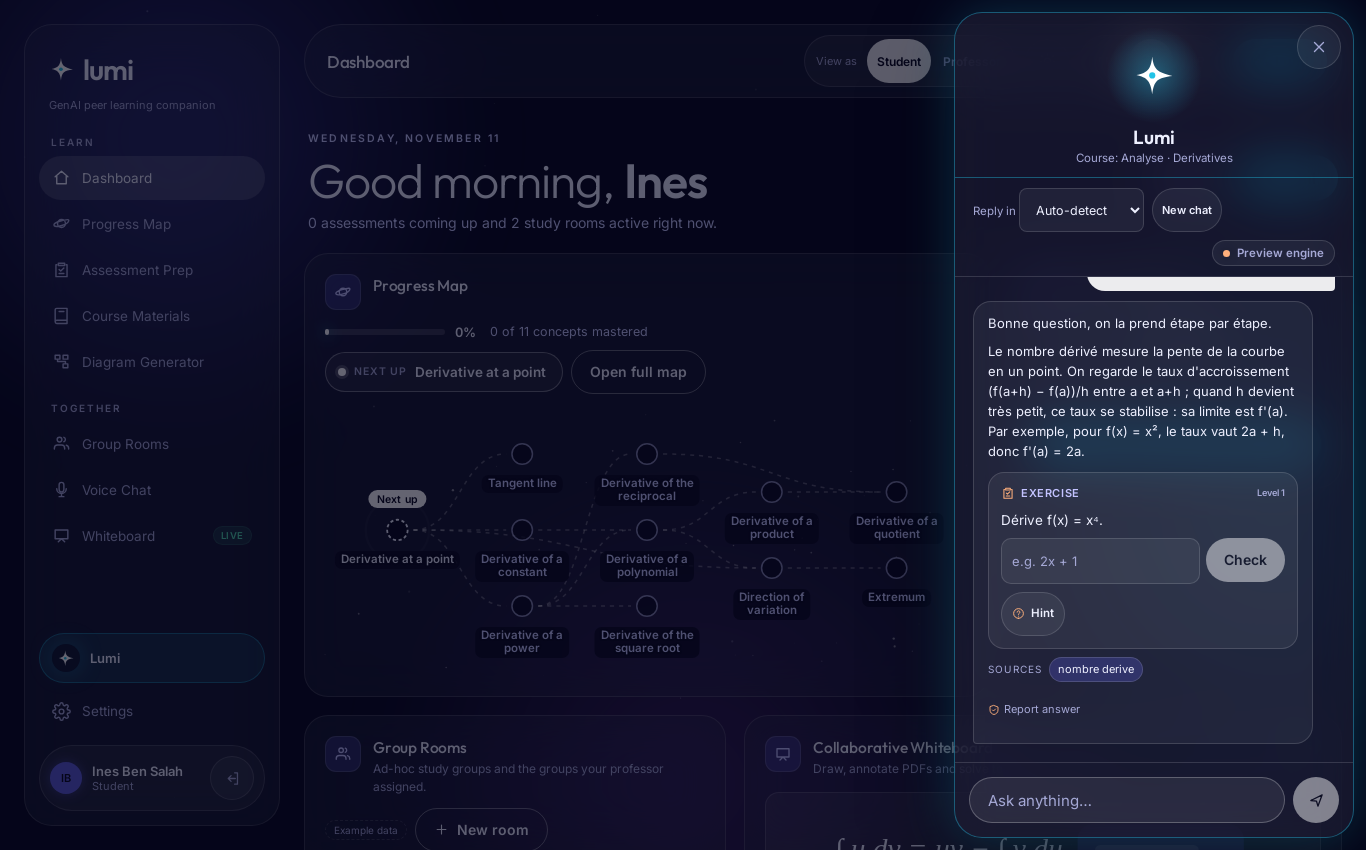
\includegraphics[width=0.495\textwidth]{../screenshots/04b-companion-answer.png}\hfill
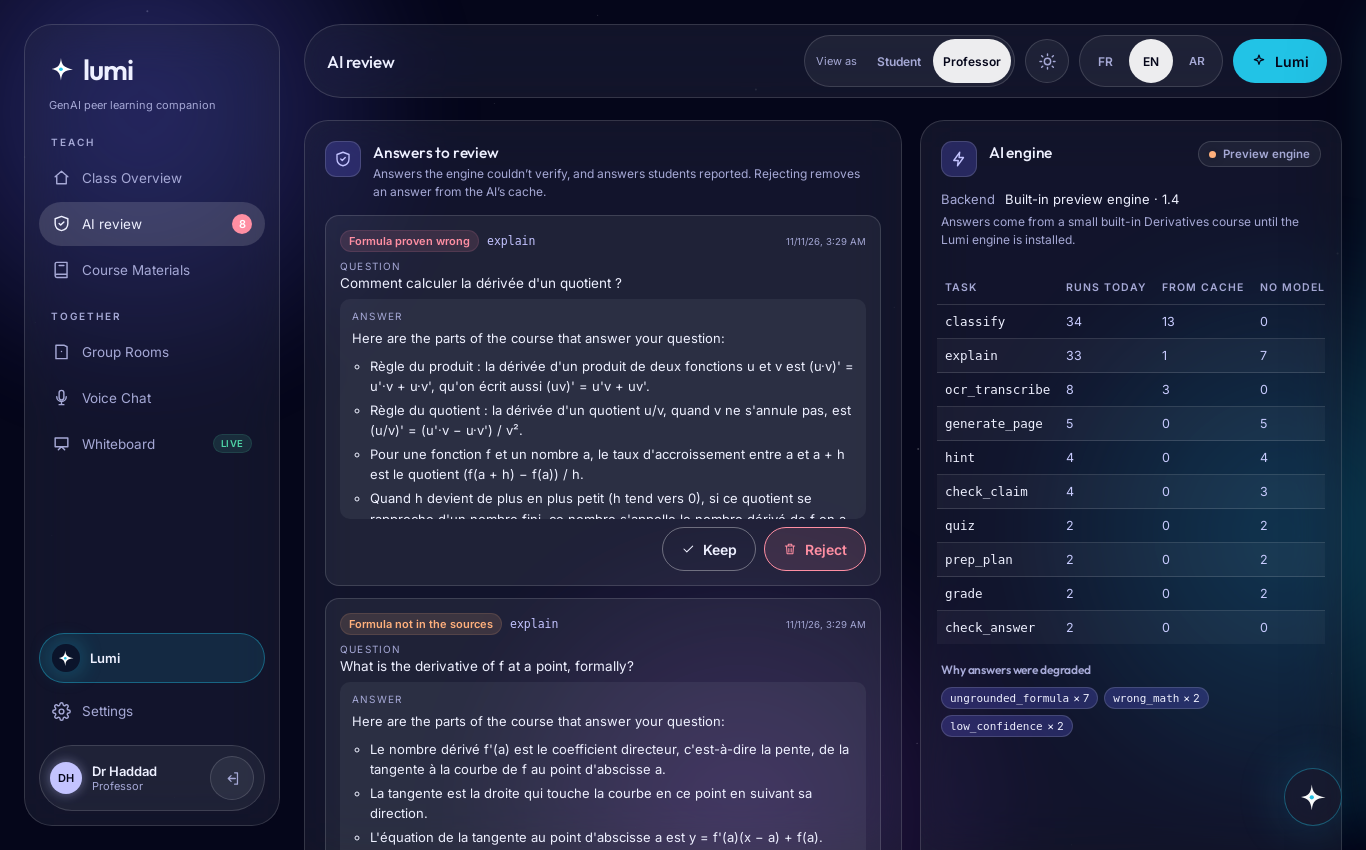
\includegraphics[width=0.495\textwidth]{../screenshots/08-professor-review.png}
\caption{Left: the companion's answer with its practice exercise and source, over the dashboard and progress map. Right: the professor's review queue and the engine's usage per task.}
\end{figure}
\vspace{-6pt}

\section{System architecture}

\begin{figure}[H]
\centering
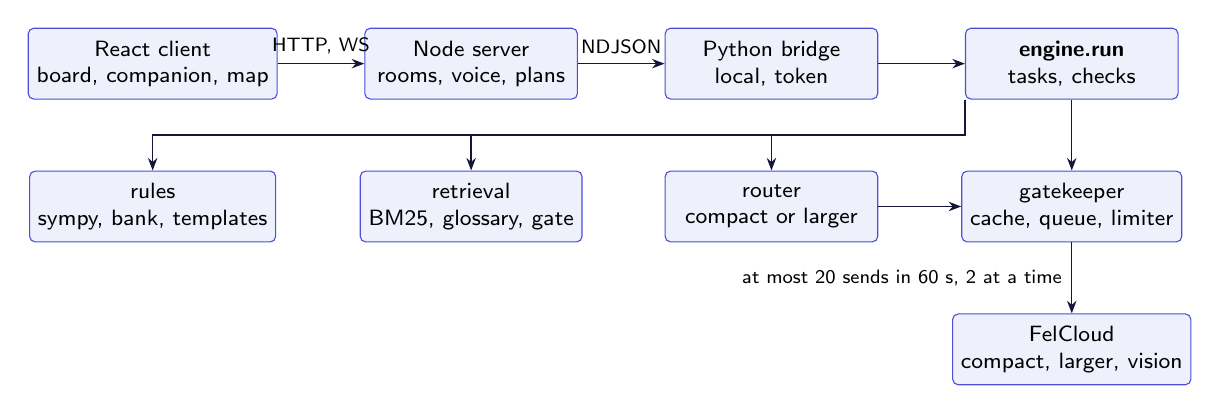
\begin{tikzpicture}[font=\sffamily\footnotesize, node distance=9mm and 11mm,
  box/.style={draw=iris, rounded corners=2pt, fill=soft, minimum height=9mm, minimum width=27mm, align=center, inner sep=3pt},
  arr/.style={-{Stealth[length=1.6mm]}, draw=ink, line width=0.5pt}]
\node[box] (client) {React client\\board, companion, map};
\node[box, right=of client] (server) {Node server\\rooms, voice, plans};
\node[box, right=of server] (bridge) {Python bridge\\local, token};
\node[box, right=of bridge] (engine) {\textbf{engine.run}\\tasks, checks};
\node[box, below=of engine] (gate) {gatekeeper\\cache, queue, limiter};
\node[box, below=of bridge] (router) {router\\compact or larger};
\node[box, below=of server] (rag) {retrieval\\BM25, glossary, gate};
\node[box, below=of client] (rules) {rules\\sympy, bank, templates};
\node[box, below=of gate] (fel) {FelCloud\\compact, larger, vision};
\draw[arr] (client) -- node[above, font=\sffamily\scriptsize]{HTTP, WS} (server);
\draw[arr] (server) -- node[above, font=\sffamily\scriptsize]{NDJSON} (bridge);
\draw[arr] (bridge) -- (engine);
\draw[arr] (engine) -- (gate);
\coordinate (bus) at ([yshift=-4.5mm]engine.south west);
\draw[arr] (engine.south west) |- (bus) -| (router.north);
\draw[arr] (bus) -| (rag.north);
\draw[arr] (bus) -| (rules.north);
\draw[arr] (router) -- (gate);
\draw[arr] (gate) -- node[left, font=\sffamily\scriptsize]{at most 20 sends in 60 s, 2 at a time} (fel);
\end{tikzpicture}
\caption{One path for every AI request. Rules and retrieval cost no request; the gatekeeper is the only code that calls the service.}
\end{figure}
\vspace{-6pt}

The client talks to a Node server (Express, Socket.IO, SQLite) that owns rooms, real-time sync, voice signalling and the
\emph{feature layer}: it adds ids, keeps exercise solutions on the server, applies plan rules and streams the engine's
progress events to the browser. A small Python bridge, bound to localhost and protected by a shared token, hosts the
engine. The engine has one entry point, \code{engine.run(task, inputs, context, priority)}, and returns the text or
parsed JSON together with the model category used, whether the answer came from the cache, whether it is degraded and
why, and the list of progress events. The provider is configuration only (base URL, key and model names per category
come from the environment), so the same code runs on FelCloud, on local models, and on a simulator that reproduces
the service's limits for tests.

\textbf{Tools.} Python 3 with asyncio, httpx, pydantic and sympy for the engine; SQLite for the cache, the metrics and
the boards; React and Canvas for the client; Node.js, Express and Socket.IO for the server; WebRTC for voice;
faster-whisper, run locally, for speech recognition. No orchestration framework sits between the application and the
models: the gatekeeper is about 1{,}600 lines of our own code, with a unit test for each part.

\subsection*{One session, counted}

Table~\ref{tab:session} is one learner's session and a professor's upload played through the application on the real
service: eight provider requests for eight steps, because classification is one call, practice is graded by rules
and repeated work comes from the cache.

\begin{table}[H]
\centering\small
\begin{tabularx}{\textwidth}{@{}Yp{3.4cm}cc@{}}
\toprule
\textbf{Step} & \textbf{Handled by} & \textbf{Requests} & \textbf{Seconds} \\
\midrule
A question in French: classified, then explained with sources & compact, then larger & 2 & 26.2 \\
A question in Arabizi, explained from the French course & larger & 1 & 10.2 \\
An exercise answered wrong, then right; mastery updated & sympy & 0 & 0.1 \\
A worked solution on the board with one wrong line & rules, compact & 1 & 4.7 \\
A two-part claim fact-checked, each part judged on its own & sympy, compact & 1 & 4.2 \\
A photo of a formula read into text & vision & 1 & 12.8 \\
One revision page: explanation, worked example, three quiz items & larger, rules & 1 & 18.5 \\
A professor's notes uploaded, then a question answered from them & larger & 1 & 8.8 \\
\bottomrule
\end{tabularx}
\caption{An end-to-end session on FelCloud, 3 November 2026: 8 requests, no refusal from the service.}\label{tab:session}
\end{table}
\vspace{-6pt}

\section{AI models and how the two categories are combined}

The service offers compact models (\code{llama3.2-3b}, \code{qwen2.5-3b}), a larger model (\code{llama3.1-8b}) and a
vision model (\code{deepseek-ocr}), all on CPU, through an OpenAI-compatible API without streaming. There is no
fine-tuning: behaviour comes from prompts, the context supplied, the choice of category and the architecture around
the models. The rule is in one file (\code{router/policy.py}); Table~\ref{tab:routing} is that rule.

\begin{table}[H]
\centering\small
\begin{tabularx}{\textwidth}{@{}p{5.6cm}p{2.3cm}Y@{}}
\toprule
\textbf{Step} & \textbf{Category} & \textbf{Reason} \\
\midrule
Classify a message: intent, language, confusion, complexity, one JSON call & compact & Short and well defined; one call instead of four \\
Hint, grading feedback, context compression, fact-check verdict, guiding question & compact & Short output with a schema, validated and repaired once \\
Explanation of a concept from retrieved course text & larger & Multi-source synthesis and careful writing; falls back to compact \\
Photo or scanned page to text & vision & The only category that reads images \\
Exercise choice, grading, formula checks, revision plan, diagrams & none & sympy and rules are exact and cost no request \\
\bottomrule
\end{tabularx}
\caption{Which category handles which step.}\label{tab:routing}
\end{table}
\vspace{-6pt}

Three design choices keep the larger model for what needs it. \emph{Rules first}: a derivative stated in words or
symbols is verified by sympy, a bank exercise is graded symbolically, a revision plan is computed; in a simulated
classroom of 96 interactive requests only 32 reached the service. \emph{The model writes only the body}: the opening
line, the exercise and the ``not in the course'' message are templates in the learner's language, so the larger model
spends its 350 output tokens on the explanation. \emph{Escalation is explicit}: a request goes to the larger model by
task, by the classifier's complexity score, or because the caller asks; never ``to be safe''.

\section{Retrieval (RAG) workflow}

\begin{enumerate}
\item \textbf{Ingest.} Course pages and professor uploads are split by heading into chunks of at most 300 tokens.
Scanned pages are read by the vision model at background priority. Each chunk carries its course, its visibility
(everyone, one class, or its uploader only) and a concept tag; a tag that is only guessed is marked for the professor
to confirm and is not used to pick exercises.
\item \textbf{Expand.} A curated glossary maps Darija, Arabizi, Arabic and English terms to the French course terms
(``mochtaqa'', ``derivative'' $\rightarrow$ ``d\'eriv\'ee''). It is deterministic: no model call.
\item \textbf{Search.} BM25 over the chunks the asker may see; professor material is boosted. The service has no
embedding model, so retrieval is lexical by design and costs no quota.
\item \textbf{Gate.} A chunk passes only if it covers at least 40\% of the question's terms (weighted by rarity).
When nothing passes, the answer is ``I could not find this in the course'' and no request is spent: the model is
never asked to answer without sources.
\item \textbf{Assemble.} The two best chunks, the history and the question must fit 2{,}800 input tokens (the context
window is 4{,}096 and the service silently cuts longer prompts); if they do not, a compact call compresses the chunks.
\item \textbf{Generate and check.} The larger model writes the explanation. Every formula in it is then verified
with sympy or matched against the sources. An answer with a wrong or unsupported formula is still shown, marked as
unverified, sent to the professor's review queue and not cached as good.
\end{enumerate}

Measured on our evaluation sets: the right chunk is first for 13 of 15 French questions and in the top three for 14;
4 of 4 off-topic questions are rejected; Darija and Arabizi questions whose answer exists only in French reach it in
the top three for 8 of 8 and 6 of 6.

\begin{figure}[H]
\centering
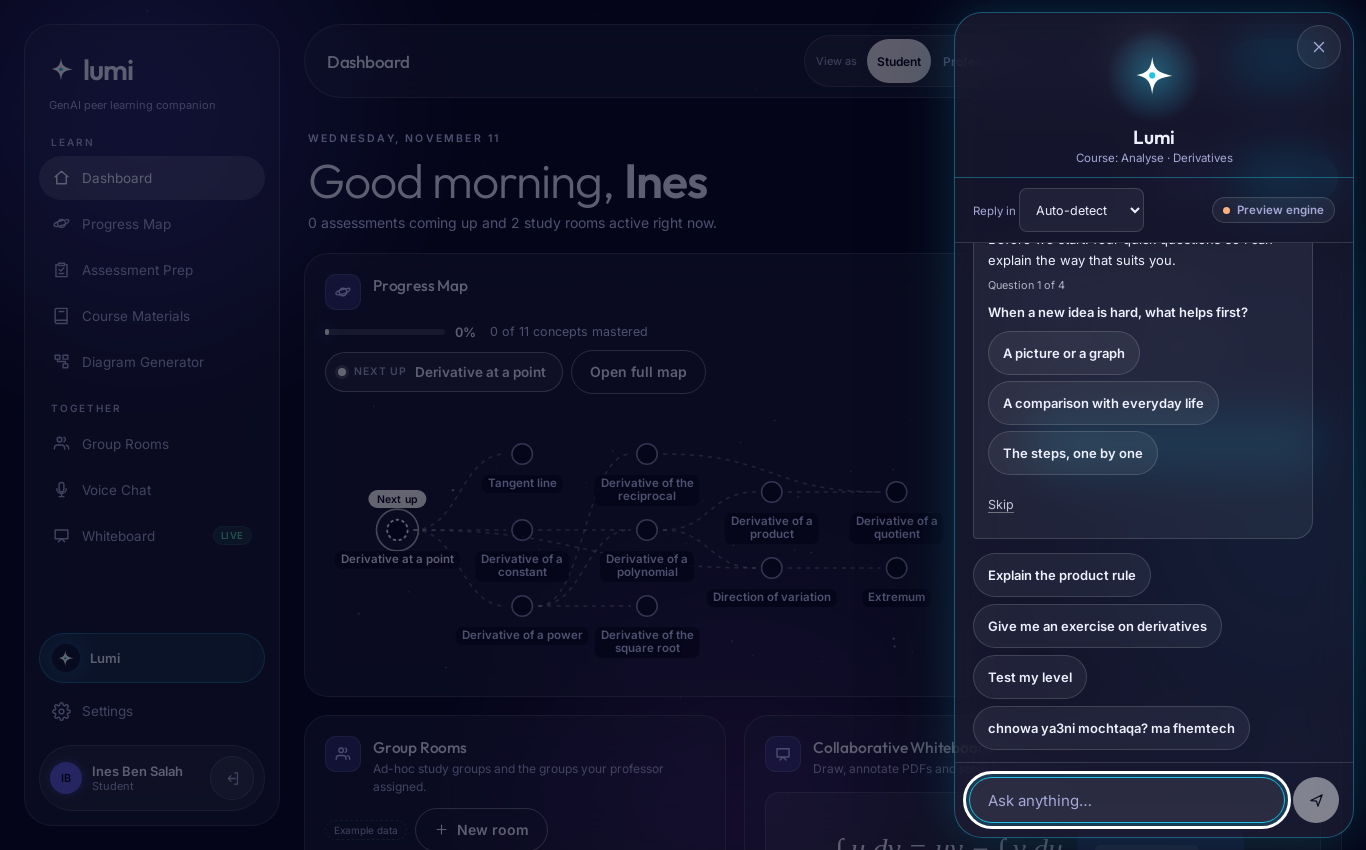
\includegraphics[width=0.495\textwidth]{../screenshots/04-learning-style-diagnostic.png}\hfill
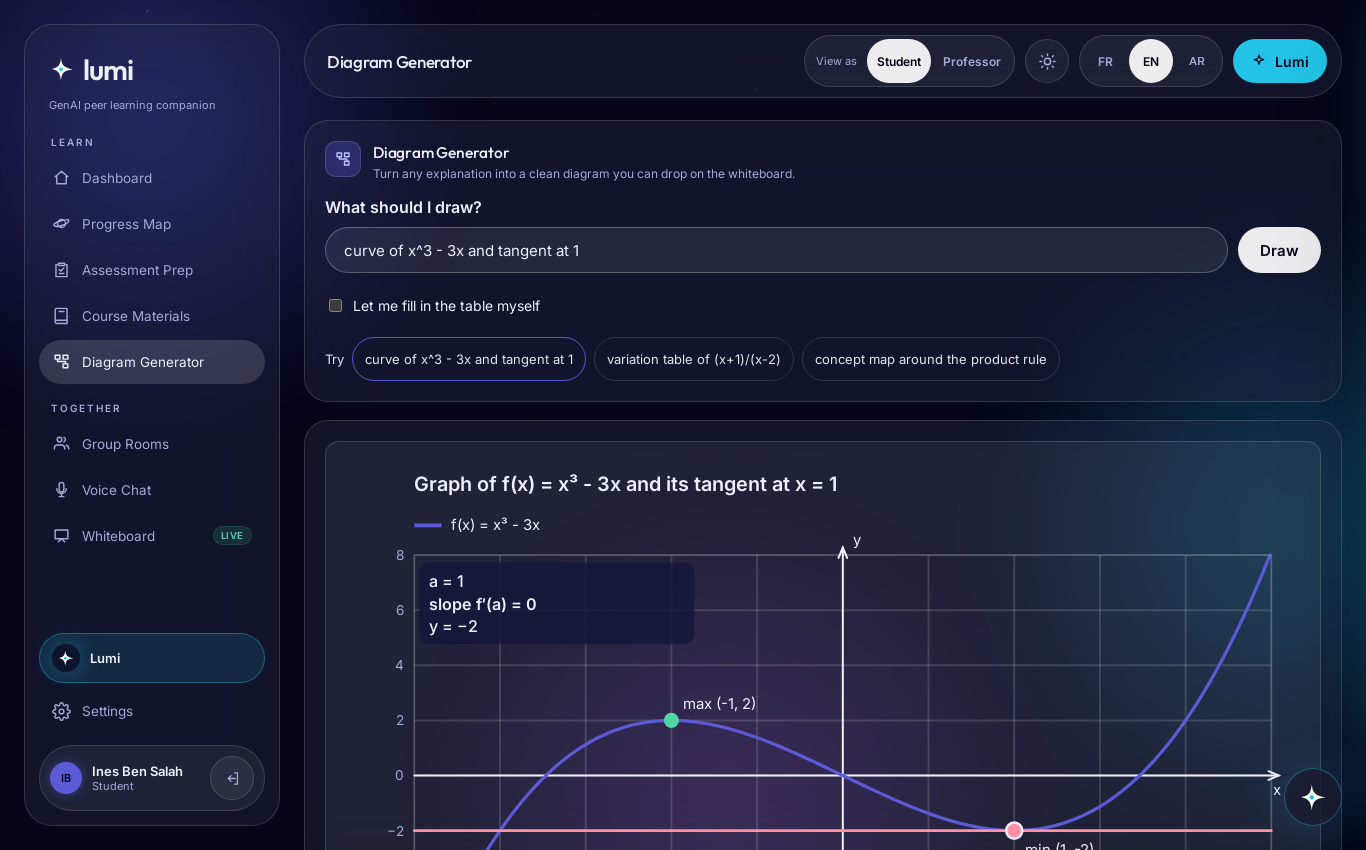
\includegraphics[width=0.495\textwidth]{../screenshots/06-diagrams.png}
\caption{Left: the diagnostic step, asked once before the first question. Right: a curve and its tangent drawn exactly from one sentence, with no model call.}
\end{figure}
\vspace{-6pt}

\section{Behaviour under limited capacity}

The service allows 20 requests in any 60 seconds and two at a time, answers in seconds to tens of seconds, and
returns whole responses. We treat these as a design budget.

\begin{table}[H]
\centering\small
\begin{tabularx}{\textwidth}{@{}p{4.6cm}Y@{}}
\toprule
\textbf{Situation} & \textbf{What the application does} \\
\midrule
Normal load & A sliding-window limiter keeps us at or under 20 sends in any 60 s; a priority queue puts a learner who is waiting ahead of background work (revision pages, OCR), and background work leaves a reserve of sends free \\
Quota refused (429 with a delay) & Waits exactly the stated delay and retries; if the wait is too long for someone watching, answers at once with the course passages and the time to come back \\
Larger model saturated or timed out & Falls back to the compact model and says so; a circuit breaker stops sending to a category that is down and probes it later with one tiny request \\
Explanation not ready in 25 s & ``Fast mode'': the retrieved passages with a one-line introduction, and a button for the full explanation \\
Same question again & Exact cache keyed by task, category, normalised prompt, language, level and style; identical concurrent requests share one call \\
An answer failed its checks & Not regenerated for 10 minutes (negative cache): the repeat gets fast mode with no request \\
Two students in one room ask at once & One AI request per room at a time; the second is told when to come back \\
No streaming & The engine emits events (checking cache, queued, retrieving, generating, falling back) that the interface shows as staged progress; a partial result is usable while the full one is written \\
\bottomrule
\end{tabularx}
\caption{Fallbacks are always visible: every result carries \code{degraded} and a reason.}
\end{table}
\vspace{-6pt}

\section{Testing strategy and results}

\textbf{Automated tests.} 1{,}153 engine tests run without any model: each gatekeeper component, the router, the
checks, and the two real refusal shapes of the service replayed from recorded fixtures. The server has 61 tests
(real-time rooms, permissions, plans, security, and the AI routes against a built-in preview engine that returns
every state of the real one) and the client 108. The API contract document is generated from real engine output and
a test fails if it drifts.

\textbf{A simulator for the limits.} Local models are too forgiving, so development runs through a constraint
simulator that reproduces latency, the quota refusal, saturation and the request ceiling.

\textbf{Measurements on the real service.}

\begin{table}[H]
\centering\small
\begin{tabularx}{\textwidth}{@{}p{5.3cm}Y@{}}
\toprule
\textbf{Run} & \textbf{Result} \\
\midrule
Offered 40 requests a minute for 60 requests (twice the limit) & 0 refusals from the service, 0 exceptions, densest 60 s window exactly 20 sends \\
Mixed classroom load, cache off, 267 s & 65 interactive requests answered with 64 provider requests (41 compact, 20 larger, 3 vision); 0 refusals, 0 exceptions; interactive latency median 2.5 s, 95th percentile 25 s; 4 of 15 explanations answered in fast mode at the deadline \\
Provider latency per step & classify 1.6--1.9 s and hint 1.8 s (compact); explanation 13--14 s median, 17--19 s at the 95th percentile (larger) \\
Classifier (compact, 3B) & intent 87\%, language 93\% on our labelled set \\
Explanations checked (91 answers) & 1 with wrong maths and 2 with a formula not in the sources, all three caught and flagged by the checker \\
Scenario run, 20 cases through the app & 15 passed at first; the 5 failures were fixed and all pass on replay (see below) \\
\bottomrule
\end{tabularx}
\caption{Results on FelCloud (October--November 2026). Reports are in the repository under \code{reports/}.}
\end{table}
\vspace{-6pt}

\subsection*{What the scenario run taught us}

We wrote 36 high-school and university scenarios and ran the 20 that need the real engine. Five failed, and each
failure was a design lesson rather than a model problem. A wrong statement in words (``the derivative of $1/x$ is
$1/x^2$'') was sent to the compact model, which answered ``not in the course''; sympy now decides it and returns the
correct form. A computer-science question was classified as a request for a quiz and received a derivative exercise;
a quiz is now served only when the message asks for one. An English question stopped at a weak English page instead
of the French definition; the search now compares both. A reply requested in English came back in French; the
language is now the last line of the prompt. Polite filler (``I don't understand\ldots can you explain?'') pushed an
on-topic question under the relevance gate; such words no longer count.

\textbf{Not done yet.} We have not tested with real learners; voice was tested with synthetic and team voices only;
Darija answers are often written in French; handwriting was tried on typed and synthetic images, not on phone
photos. The class figures on the professor's overview are partly example data and are labelled as such.

\section{Privacy and ethical safeguards}

\begin{itemize}
\item \textbf{Little personal data.} There are no real accounts: a learner picks a display name and a role, and the
browser gets a random id. The display name is shown to the other members of a room and stored with a file the learner
uploads; the email typed at sign-in stays in the browser and no password is stored. Tests, fixtures and course text
are synthetic or public.
\item \textbf{What reaches the inference service.} Course text, the question with the recent turns of the conversation,
the text on the board, the text of an uploaded file when an answer uses it, and a photo or scanned page when it is
read. Never a name, an email or an id: in voice, speakers are sent as ``Student 1'', ``Student 2''.
\item \textbf{Voice.} Group audio is peer to peer and is not recorded. A spoken question is transcribed on our own
server by a local speech model, used once and discarded.
\item \textbf{Credentials.} Keys exist only in git-ignored environment files; the repository ships a template with
placeholders, and reports are scanned for key-like strings before they are written.
\item \textbf{The AI supports the teacher.} Professor material ranks first; unverified answers go to a review queue;
a professor can remove an answer from the cache; the companion gives hints before solutions.
\item \textbf{Fairness.} All five languages get the same pipeline and the same checks; the level of an exercise comes
from the learner's own answers, never from a profile. One request per room at a time keeps one person from taking
the group's quota.
\item \textbf{Honesty about limits.} ``Not in the course'' instead of an invented answer; every fallback is shown.
\item \textbf{Application security.} Uploads must match their declared type and are served back inert; the API sends
strict security headers; room codes are hashed; inputs are validated and rate limited.
\end{itemize}

\section{Business-model note}

\textbf{Target users.} Private universities and training centres with 100 to 1{,}000 learners come first: they can
pay, decide faster than public systems, and teach the first-year content Lumi has today. Independent tutors and
individual learners arrive through self-service; high schools follow once safeguards for minors are in place.

\textbf{Value proposition.} Course-grounded help in the student's language, with the educator in control. Against a
free general assistant, Lumi answers from the professor's material, checks the maths, and gives the professor a
review queue and concept-level insight. Against the learning-management system an institution already runs, Lumi is
a layer added to it, not a replacement.

\textbf{Adoption path.} A capped free tier brings students and tutors in; their use is the evidence for a paid pilot
with one department on real course material and agreed success measures; the pilot becomes an annual licence. The
institution keeps its LMS: launching Lumi from a course (LTI 1.3), roster sync and grade return are the planned
integration, with file import as the first step.

\begin{table}[H]
\centering\small
\begin{tabularx}{\textwidth}{@{}p{2.2cm}p{3.6cm}Y@{}}
\toprule
\textbf{Plan} & \textbf{For} & \textbf{What it includes} \\
\midrule
Free & Individual learners & Companion capped at 30 AI requests a day, whiteboard and voice without AI, one exam in assessment prep \\
Educator & Tutors, small cohorts & Everything with AI, class material, answer review (subscription) \\
Campus & Institutions & The same with institutional administration and the standard LMS connector (annual licence) \\
Enterprise & Networks & Custom integrations and service commitments (contract) \\
\bottomrule
\end{tabularx}
\caption{Plans. The feature rules of this table are already enforced by the server as a preview; billing is not built.}
\end{table}
\vspace{-6pt}

\textbf{Sustainability.} Planning assumptions, not yet tested with buyers: 40 TND per learner per year and a
1{,}500 TND onboarding fee, so one pilot of 200 learners is 9{,}500 TND in the first year and five institutions of
500 learners are 107{,}500 TND. At a 70\% gross margin the direct cost ceiling is 12 TND per learner per year, about
1 TND a month, which is why the engineering in this report matters commercially: rules before models, the compact
model before the larger one, a cache, and a cap on free use are what keep inference under that ceiling. Beyond the
hackathon the engine is provider-agnostic, so it can move to production capacity without a rewrite. The main risk is
that institutions like the product but do not see enough added value to pay; paid pilots with agreed measures are
how we test it. The next steps are verified accounts, real rosters, and a second course.

\end{document}
